% Please make sure you insert your
% data according to the instructions in PoSauthmanual.pdf
\documentclass{PoS}
\usepackage{amsmath}

\title{Baryon bag simulation of QCD in the strong coupling limit}

\ShortTitle{Baryon bag simulation of QCD in the strong coupling limit}


\author{\speaker{Oliver Orasch}\\
        University of Graz, Institute of Physics, 8010 Graz, Austria\\
        E-mail: \email{oliver.orasch@uni-graz.at}}
        
\author{Christof Gattringer\\
        University of Graz, Institute of Physics, 8010 Graz, Austria\\
        E-mail: \email{christof.gattringer@uni-graz.at}}
        
\author{Shailesh Chandrasekharan\\
        Duke University, Physics Departement, 27704 Durham, NC, USA\\
        E-mail: \email{sch@phy.duke.edu}}
        
\author{Pascal Toerek\\
        University of Graz, Institute of Physics, 8010 Graz, Austria\\
        E-mail: \email{pascal.toerek@uni-graz.at}}
        
    
\abstract{We explore the possibility of a simulation of strong coupling QCD in terms of baryon bags. Since the gauge action is missing in the strong coupling partition sum, the integration over the gauge group is possible and the remaining Grassmann integral can be mapped to a statistical system of monomers, dimers and loops. Rather recently it was shown that the contributions from the baryons, i.e., the tri-quark monomers, dimers and loops, can be collected in so-called baryon bags. Within the bags the baryons propagate freely whereas the rest of the lattice is solely filled with interacting meson terms, i.e., quark and di-quark monomers and dimers. We perform a simulation directly in the baryon bag language and show first results in two dimensions.}


\FullConference{The 37th Annual International Symposium on Lattice Field Theory - LATTICE2019\\
		16-22 June, 2019\\
		Hilton Hotel, Wuhan, Hubei, China.}


\begin{document}

\section{Introduction}

We present a method to restrict the sign problem to subsets of the lattice. Within this so-called fermion bags the sign problem is solved exactly as long as the chemical potential is small.

\section{Baryon bags and the fermion sign problem}

%In this work we revisit the idea to simulate strong coupling QCD in terms of a system of fermion worldlines.

As a starting point we would like to familiarize the reader with the model. Strong coupling QCD ($\beta = 0$) is given by the partition function
\begin{equation}
Z = \int \mathcal{D}\big[\overline{\psi}\psi\big] \int \mathcal{D}\big[U\big] \;\text{e}^{S_F\left[\overline{\psi},\psi,U\right]}
\label{eq:part_sum}
\end{equation} 
where the Grassmann and SU(3) Haar measures are given by the following product measures
\begin{equation*}
\int \mathcal{D}\big[\overline{\psi}\psi\big]  = \prod_{x} \int \prod_{a = 1}^{3}\text{d}\overline{\psi}_{x,a}\text{d}\psi_{x,a} \;\;\;\text{ and } \;\;\;\int \mathcal{D}[U] = \prod_{x,\nu} \int_{\text{\tiny SU(3)}} \text{d}U_{x,\nu}.
\end{equation*}
Furthermore, we use one flavor of staggered quarks realized by the action
\begin{equation}
S_F\left[\overline{\psi},\psi,U\right] = \sum_x\Big(2m\overline{\psi}_x \psi_x + \sum_{\nu} \xi_{x,\nu}\Big[ \text{e}^{\mu\delta_{\nu, d}}\overline{\psi}_{x} U_{x,\nu} \psi_{x+\hat{\nu}} - \text{e}^{-\mu\delta_{\nu, d}}\overline{\psi}_{x+\hat{\nu}}U^{\dagger}_{x, \nu} \psi_{x} \Big] \Big).
\label{eq:stag_act}
\end{equation}
The quark fields $\psi_x$ $(\overline{\psi}_x)$ are 3-component Grassmann vectors, each component representing a color. They live on the sites of a $d$ dimensional lattice of volume $V = N_s^{d-1}N_t$. The SU(3) valued gauge fields $U_{x,\nu}$ live on the links of the aforementioned lattice. For the fermions, we choose periodic boundary conditions in spatial ($\nu = 1,\dots, d-1$) and anti-periodic boundary conditions in temporal ($\nu = d$) direction. We take the boundary conditions of the gauge links to be periodic in all directions. Since we are interested in driving the temperature we include an anisotropic coupling for the temporal direction. Together with the staggerd sign functions, we incorporate the bare anistropic coupling $t$ in the link factor $\xi_{x,\nu} = t^{\delta_{\nu,\pm d}}\gamma_{x,\nu}$, where the staggered signs $\gamma_{x,\nu}$ are defined as usual,
\begin{equation}
\gamma_{x, 1} = 1, \hspace*{0.5cm}\gamma_{x, 2} = (-1)^{x_1},\;\; \dots, \hspace*{0.5cm}\gamma_{x, d} = (-1)^{x_1 + \dots + x_{d-1}}.
\end{equation}
Conventionally, the staggered action is defined with a factor of $1/2$ in front of the kinetic term. For conveniece, however, we rescaled the fermion fields by a factor of $\sqrt{2}$ yielding (\ref{eq:stag_act}). In principle, it is also possible to include a quark chemical potential $\mu$. In a conventional representation, however, this leads to a finite density sign problem.\\
\\
Let us briefly introduce the baryon bag representation. We refrain from giving a full derviation of the baryon bag partion sum and redirect the interested reader to \cite{Gattringer:2018mrg} where the mapping procedure was discussed rigorously. Here, we would rather give an intuitive illustration on the basis of the worldline representation of strong coupling QCD proposed by Karsch and M\"utter \cite{Karsch:1988zx}
\begin{equation}
Z = \sum_{\{n, d, \ell\}} w_n(m) \; w_d(t) \; w_{\ell}(\mu,t).
\end{equation}
The worldline degrees of freedom in this representation are monomers $n_x$ ($\hat{=}$ mass terms), dimers $d_{x,\nu}$ ($\hat{=}$ a forward hop followed by an backward hop on the same link) and baryon loops $\ell_{x,\nu}$ ($\hat{=}$ consecutive non-(self)intersecting forward/backward hops on a closed contour). Baryon loops are fermion loops of three quarks propagating coherently and, hence, $\ell_{x,\nu}$ is either $0$ or $1$. The occupations for the monomer are $n_x = 0,1,2,3$ and the dimers $d_{x,\nu} = 0,1,2,3$. Furthermore, an admissible configuration must satisfy the Grassmann constraint
\begin{equation}
n_x + \sum_{\nu} d_{x,\nu} + \sum_{\nu} \frac{3}{2} |\ell_{x,\nu}| = 3.
\label{eq:GM_const}
\end{equation}
In principle, monomers and dimers carry color. This information, however, can be absorbed in combinatorical factors \cite{Rossi:1984cv, Karsch:1988zx, Marchis:2018tcs}.\\
\\
As it stands, partition sum (\ref{eq:part_sum}) is not suitable for a Monte Carlo simulation. Due to the fermion sign problem the weights of the baryon loops, $w_{\ell}(\mu,t)$, are not strictly posititive, not even for $\mu = 0$. Therefore, we need to group sets of configurations in such a way that the collective weights are appropriate for simulation. In the following we will use a fermion bag strategy \cite{Chandrasekharan:2009wc} to obtain real and positive weights in the partition sum. The first observation is that baryonic degrees of freedom, i.e., 3-monomers ($n_x = 3$), 3-dimers ($d_{x,\nu}=3$) and baryon loops, trivially saturate the Grassmann constraint (\ref{eq:GM_const}). According to this observation each worldline configuration can be decomposed into baryon clusters and regions filled with mesonic degrees of freedom. Thus, for fixed background all configurations can be classified according to the baryon cluster structure. If we sum up all configurations belonging to the same class we obtain a non-local description where fermions are restricted to clusters of arbitrary shape. With a careful analysis of the strong coupling partition sum, it is possible to show that the physics within these clusters is described by a free staggered action 
\begin{equation}
S_B\left[\overline{B},B\right] = \sum_x\Big(2M\overline{B}_x B_x +\sum_{\nu} \xi_{x,\nu}^3\Big[ \text{e}^{3\mu\delta_{\nu,d}}\overline{B}_{x} B_{x+\hat{\nu}} - \text{e}^{-3\mu\delta_{\nu,d}}\overline{B}_{x+\hat{\nu}}B_{x} \Big] \Big)
\label{eq:baryon_act}
\end{equation}
where $M = 4m^3$ is the bare baryon mass for the composite baryon field $B_x = \psi^{1}_x\psi^{2}_x\psi^{3}_x$ ($\overline{B}_x = \overline{\psi}^{3}_x\overline{\psi}^{2}_x\overline{\psi}^{1}_x$). In the following we will referr to such a cluster as a baryon bag. Each bag $\mathcal{B}_i$ which can occupy any arbitrary region on the lattice has a weight of
\begin{equation}
\text{det} D[\mathcal{B}_i]  = \int\limits_{\mathcal{B}_i} \prod_{x\in\mathcal{B}_i} \text{d} B_x \text{d}\overline{B}_x \exp\Big(\sum\limits_{x,y \in \mathcal{B}_i} \overline{B}_x D^{(i)}_{xy} B_y\Big)
\label{eq:baryon_det}
\end{equation}
where $D^{(i)}_{xy}$ is the free Dirac operator defined by the baryon action (\ref{eq:baryon_act}). In (\ref{eq:baryon_det}) each loop is paired with a compatible 3-dimer chain and $\text{det} D[\mathcal{B}_i] \geq 0$. The latter condition only holds for small $\mu$.\\
The union of all bags $\mathcal{B} = \cup_i \mathcal{B}_i$ we call the bag region. The rest of the lattice is filled with mesonic contributions - this region we denote as the complementary domain $\overline{\mathcal{B}}$. It is occupied by networks of  monomers and dimers with $n_x = 0,1,2$ and $d_{x,\nu} = 0,1,2$. Thus, the parition sum for strong coupling QCD in the baryon bag representation is given by
\begin{equation}
Z = \sum_{\{\mathcal{B}\}}\prod_{\mathcal{B}_i \in \mathcal{B}} \text{det}D[\mathcal{B}_i] \; \times \; Z_{\overline{\mathcal{B}}}
\end{equation}
where $Z_{\overline{\mathcal{B}}} = \sum_{\{n, d || \mathcal{B}\}} w_n(m) \; w_d(t)$ is the weight for the complementary domain. The set $\{n, d || \mathcal{B}\}$ denotes the set of $\overline{\mathcal{B}}$ configurations that are compatible with a given bag structure $\mathcal{B}$. See figure ... for a typical configuration of this system.\\
\\
Finally, let us comment on the difference to the simulation strategy of Karsch and M\"utter \cite{Karsch:1988zx}. To circumvent the fermion sign problem, Karsch and M\"utter proposed to sample U(3) configurations and then reweight each U(3) configuration to the corresponding SU(3) configuration. Since U(3) and SU(3) merely differ by the presence fermion loops they proposed to identify closed contours of alternating 1- and 2-dimers. These contours are then viewed as a superposition of dimer chain and fermion loop and thus solve the sign problem. In a brief comment in \cite{Karsch:1988zx} it was also mentioned that a reweighting to chains of 3-dimers would in principle be possible. However, it was argued that the choice of the contour of the loop might not be unique for a given dimer occupation. This is exactly the role of the bag determinant: It is a quantum mechanical superposition of all possible ways to fill a given subset of the lattice with baryonic degrees of freedom: 3-monomers, 3-dimers and baryon loops. Thus, the bag representation fully takes into account the fermionic degrees of freedom of the model and simulataneously solves the fermion sign problem exactly - at least for small chemical potential.

\subsection{Observables}

The observables conventionally discussed in strong coupling QCD are the chiral condensate and the chiral susceptibility, i.e.,
\begin{equation}
\langle \overline{\psi}\psi \rangle = \partial \ln Z/\partial m / V \hspace{1cm} \text{and} \hspace{1cm} \chi_{\overline{\psi}\psi} = \partial \langle\overline{\psi}\psi\rangle/\partial m + V\langle \overline{\psi}\psi \rangle^2,
\end{equation}
where $ \chi_{\overline{\psi}\psi}$ is defined to include connected and disconnected terms. Furthermore, in the baryon bag picture an interesting observable is accessible: the average bag size $S_B$. Its expectation value is defined as
\begin{equation}
\langle S_B \rangle = (1/V) \sum_{\mathcal{B}_i \in \mathcal{B}} |\mathcal{B}_i|
\end{equation}
where $|\mathcal{B}_i|$ denotes the sites in the i-\textit{th} bag. It is a measure for the fraction of the lattice where the physics is described by the baryon action (\ref{eq:baryon_act}). Loosely speaking, it measures the distribution of degrees of freedom of the system. In the following, we will always compare a conventional observable - the condensate or the susceptibility - with the bag size to see if a change in the observabe is signaled in the change of worldline degrees of freedom.
\subsection{Algorithm}

In this work we use two kinds of algorithms: For a proof-of-concept study in 2D we use local algorithm that tries to exchange a dimer with a pair of monomers and vice versa. See \cite{Karsch:1988zx}. Albeit this algorithm breaks down in the chiral limit, it works well with the bag representation. In the following \textit{bag simulation} refers to this strategy.\\
\\For cross-checking and simulation on large lattices/higher dimensions we also developed a new worm algorithm. Basically, it is a natural extension of the well-known U(3)-worm \cite{Adams:2003cca} to arbitrary $m$. We postpone a detailed description and proof of detailed balance to future publications \cite{Orasch:2019_1, Orasch:2019_2}. Here we explain the algorithm for U(N).\\
At first we pick a site $x$ with a probaility of $1/V$. Due to the presence of monomers, the worm may start in two ways: With a probabililty of $n_x/N$ the worm starts at the site by naming a monomer \textit{head}. With probability $d_{x,\nu}/N$ the worm decreases $d_{x,\nu}$ by $1$. To meet the Grassmann constraint, the algorithm increases $n_x$ by 1 and puts the \textit{head} onto the site $x+\hat{\nu}$. For convenience we introduce $t_{\nu} = t^{\delta_{\nu,\pm d}}$ and $w = 2(d-1) + 2t^2 + (2m)^2$. Once the worm has started it exits on the site with a probability $(2m)^2/w$ (by replacing \textit{head} with a monomer) or moves with probability $t^2_{\nu}/w$ in the direction $\nu$. By doing so the head temporarily moves to an intermediate site $x+\hat{\nu}$ by increasing $d_{x,\nu}$ by $1$. The worm has again two options: Exiting at this particular site with probability $n_{x+\hat{\nu}}/(N-d_{x,\nu})$ by decreasing $n_{x+\hat{\nu}}$ by $1$ or moving the \textit{head} to an adjacent site with probability $d_{x+\hat{\nu}, \mu}/(N-d_{x,\nu})$ by decreasing $d_{x+\hat{\nu}, \mu}$ by $1$. Thus, by moving the worm shuffles the monomer and dimer configuration and by combining the various starting/closing steps it is able to raise/lower the monomer number in steps of $2$. Note, that despite the fact that we defined a \textit{head} we did not mention a \textit{tail}. In this description any monomer is considered a \textit{tail} meaning the worm has the option to exit any time a monomer is encountered.\\
As described in \cite{Adams:2003cca}, the weights of the worm configurations are defined in such a way that the U(N) condensate is simply given by the length $L$ of the worm. To get the corresponding SU(N) observables we need to employ a Karsch-M\"utter-type reweighting strategy as described above. We use \cite{Boyd:1991fb}
\begin{equation}
\langle \mathcal{O} \rangle_{\tiny SU(3)} = \frac{\langle \mathcal{O} \prod_{\ell}(1 + f_{\ell}(t)\text{ sign}(\ell)) \rangle_{\tiny U(3)}}{\langle \prod_{\ell}(1 + f_{\ell}(t)\text{ sign}(\ell)) \rangle_{\tiny U(3)}}
\end{equation}
where $f_{\ell}(t) = 2/(t^{n^{\ell}_t} + t^{-n^{\ell}_t})$ with $n^{\ell}_t = 3N^{\ell}_t - 2N^{\ell}_{Dt}$. $N^{\ell}_t$ is the number of loop segements and $N^{\ell}_{Dt}$ is the number of dimers in time direction. In the following, we call this strategy \textit{worm simulation}.

\section{2D Results}

Firstly, we cross-check the results from the \textit{bag simulation} on small lattices. On a $2x2$ we can systematically count all possible configurations and, thus, provide exact results to confront our data. 
\begin{figure}
\centering
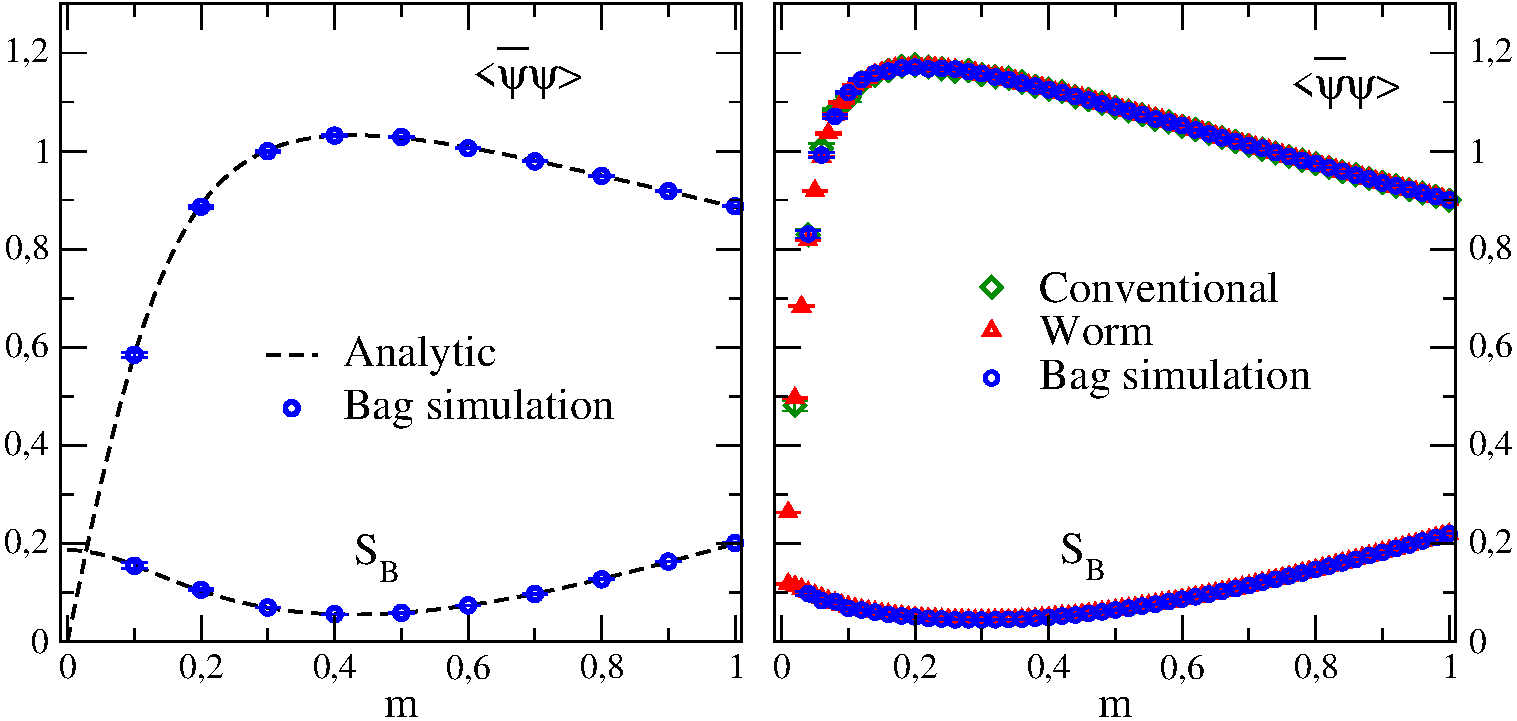
\includegraphics[width=0.7\linewidth]{Plots/Checks/Comb/V2n4_SB_cond_m0to1_combined.pdf}
\caption{Cross-checks for the condensate and the bag size. Blue circles denote the data from the \textit{bag simulation} in both panels. \textit{(Left)} $V = 2x2$; the dashed line is data from an exact counting of configurations. \textit{(Right)} $V = 4x4$; Red triangles denote data from the \textit{worm}, green diamonds data from a conventional simulation.}
\label{fig:check}
\end{figure}
Since $2x2$ is extremely small, some configurations are not possible that automatically appear on larger lattices.  Therefore, we also cross-check on a $4x4$ lattice. In this case counting the configurations is not an option and we use the \textit{worm}. Additionally, we augment (at least for the condesate) the check by including data from a conventional simulation. See Figure (\ref{fig:check}). The left panel shows the data for the $2x2$ lattice; the right panel the $4x4$ case. The data matches nicely the reference data and we conclude that both the \textit{bag} and the \textit{worm simulation} have been implemented correctly.

\newpage

\section{4D Results}

\newpage


\section{Concluding remarks}

\section{Acknowledgment}
O. Orasch would like to thank Duke University for their hospitality where a large part of this work was conducted. Furthermore, O. Orasch thanks the Austrian Marshallplan Foundation for financial support.
 

\begin{thebibliography}{99}

%\cite{Rossi:1984cv}
\bibitem{Rossi:1984cv} 
  P.~Rossi and U.~Wolff,
  %``Lattice {QCD} With Fermions at Strong Coupling: A Dimer System,''
  Nucl.\ Phys.\ B {\bf 248}, 105 (1984).
 % doi:10.1016/0550-3213(84)90589-3
  %%CITATION = doi:10.1016/0550-3213(84)90589-3;%%
  %114 citations counted in INSPIRE as of 11 Jul 2019
  
%\cite{Wolff:1984we}
\bibitem{Wolff:1984we} 
  U.~Wolff,
  %``Baryons in Lattice {QCD} at Strong Coupling,''
  Phys.\ Lett.\  {\bf 153B}, 92 (1985).
  doi:10.1016/0370-2693(85)91448-0
  %%CITATION = doi:10.1016/0370-2693(85)91448-0;%%
  %26 citations counted in INSPIRE as of 11 Jul 2019

%\cite{Karsch:1988zx}
\bibitem{Karsch:1988zx} 
  F.~Karsch and K.~H.~M\"utter,
  %``Strong Coupling Qcd At Finite Baryon Number Density,''
  Nucl.\ Phys.\ B {\bf 313}, 541 (1989).
  %doi:10.1016/0550-3213(89)90396-9
  %%CITATION = doi:10.1016/0550-3213(89)90396-9;%%
  %129 citations counted in INSPIRE as of 11 Jul 2019

%\cite{Boyd:1991fb}
\bibitem{Boyd:1991fb} 
  G.~Boyd, J.~Fingberg, F.~Karsch, L.~Karkkainen and B.~Petersson,
  %``Critical exponents of the chiral transition in strong coupling QCD,''
  Nucl.\ Phys.\ B {\bf 376}, 199 (1992).
  %doi:10.1016/0550-3213(92)90074-L
  %%CITATION = doi:10.1016/0550-3213(92)90074-L;%%
  %41 citations counted in INSPIRE as of 11 Jul 2019
  
  %\cite{Gattringer:2018mrg}
\bibitem{Gattringer:2018mrg} 
  C.~Gattringer,
  %``Baryon bags in strong coupling QCD,''
  Phys.\ Rev.\ D {\bf 97}, no. 7, 074506 (2018)
%  doi:10.1103/PhysRevD.97.074506
 % [arXiv:1802.09417 [hep-lat]].
  %%CITATION = doi:10.1103/PhysRevD.97.074506;%%
  %2 citations counted in INSPIRE as of 18 Jul 2019
  
%\cite{Chandrasekharan:2009wc}
\bibitem{Chandrasekharan:2009wc} 
  S.~Chandrasekharan,
  %``The Fermion bag approach to lattice field theories,''
  Phys.\ Rev.\ D {\bf 82}, 025007 (2010)
%  doi:10.1103/PhysRevD.82.025007
%  [arXiv:0910.5736 [hep-lat]].
  %%CITATION = doi:10.1103/PhysRevD.82.025007;%%
  %61 citations counted in INSPIRE as of 23 Jul 2019
  
  %\cite{Marchis:2018tcs}
\bibitem{Marchis:2018tcs} 
  C.~Marchis, C.~Gattringer and O.~Orasch,
  %``Bag representation for composite degrees of freedom in lattice gauge theories with fermions,''
  PoS LATTICE {\bf 2018}, 243 (2018)
%  doi:10.22323/1.334.0243
%  [arXiv:1811.09372 [hep-lat]].
  %%CITATION = doi:10.22323/1.334.0243;%%
  
  %\cite{Creutz:1978ub}
\bibitem{Creutz:1978ub} 
  M.~Creutz,
  %``On Invariant Integration Over Su(n),''
  J.\ Math.\ Phys.\  {\bf 19}, 2043 (1978).
%  doi:10.1063/1.523581
  %%CITATION = doi:10.1063/1.523581;%%
  %82 citations counted in INSPIRE as of 18 Jul 2019
  
  %\cite{Adams:2003cca}
\bibitem{Adams:2003cca} 
  D.~H.~Adams and S.~Chandrasekharan,
  %``Chiral limit of strongly coupled lattice gauge theories,''
  Nucl.\ Phys.\ B {\bf 662}, 220 (2003)
 % doi:10.1016/S0550-3213(03)00350-X
  %[hep-lat/0303003].
  %%CITATION = doi:10.1016/S0550-3213(03)00350-X;%%
  %69 citations counted in INSPIRE as of 19 Jul 2019
  
%\cite{Orasch:2019_1}
\bibitem{Orasch:2019_1} 
 O.~Orasch and S.~Chandrasekharan,
	work in preparation
	
%\cite{Orasch:2019_2}
\bibitem{Orasch:2019_2} 
 O.~Orasch, C.~Gattringer and S.~Chandrasekharan,
 work in preparation



\end{thebibliography}

\end{document}
